\documentclass[conference]{IEEEtran}
\IEEEoverridecommandlockouts
% The preceding line is only needed to identify funding in the first footnote. If that is unneeded, please comment it out.
\usepackage{cite}
\usepackage{amsmath,amssymb,amsfonts}
\usepackage{graphicx}
\usepackage{textcomp}
\usepackage{xcolor}
\def\BibTeX{{\rm B\kern-.05em{\sc i\kern-.025em b}\kern-.08em
    T\kern-.1667em\lower.7ex\hbox{E}\kern-.125emX}}
\title{
\vspace{1cm}
{
\includegraphics[width=0.15\textwidth]{iithlogo.jpg} \\ ESP-32 Assignment} }
\author{Akkugari Ruchika \\ Roll No: FWC22276 \\ akkugariruchika@gmail.com}
 \begin{document}
\maketitle
 \section {ABSTRACT}
 A $4-bit$ priority encoder has inputs $D_3, D_2, D_1$ and $D_0$ in descending order of priority. The two-bit output $AB$ is generated as $00, 01, 10$ and $11$ corresponding to inputs $D_3, D_2, D_1$ and $D_0$, respectively. The Boolean expression of the output bit $B$ isto be implemented.
 \begin{figure}[h]
	 \centering
	 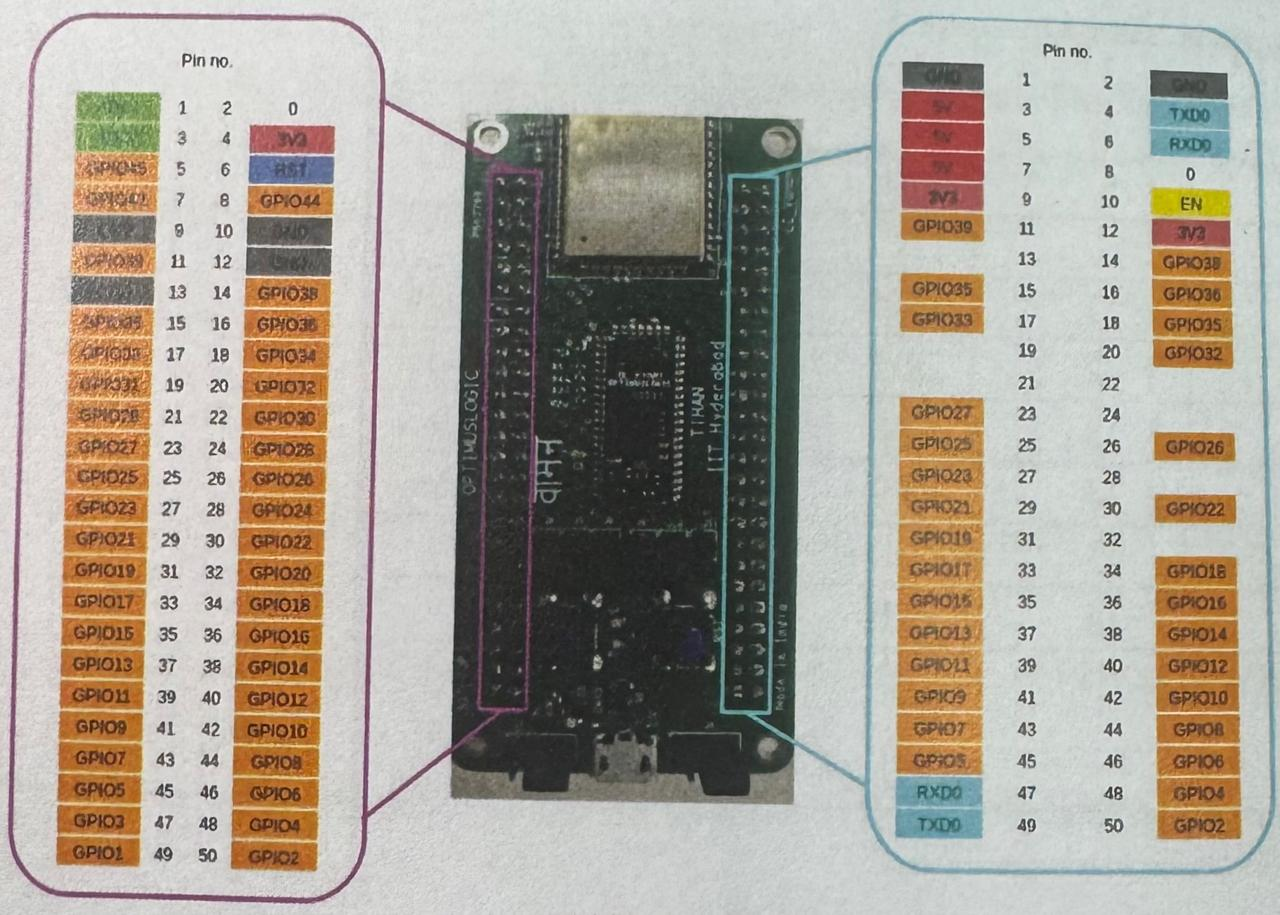
\includegraphics[width=0.35\textwidth]{vaman.jpg}
	 \caption{\label{fig:Esp-32 in vaman board}}
 \end{figure}
\section{COMPONENTS}
The required components list is given in Table: I. 
 \begin{table} [htbp]
\centering
\begin{tabular}{| c | c | c |} \hline
Components & Value & Quantity \\\hline
LEDs &  & 1 \\ \hline
Arduino & UNO & 1 \\ \hline
Jumper Wires &  & 10 \\ \hline
Breadboard & & 1 \\ \hline
	Vaman Board & & 1\\
\hline
\end{tabular}
\vspace{0.1cm}
\caption{\label{tab:widgets}}
\end{table}
\section{PROCEDURE}
To set up the Boolean logic circuit on an ESP32, connect GPIO pins (e.g., GPIO15 for D3, GPIO2 for D2, GPIO4 for D1, and GPIO16 for D0) as inputs, with VCC or GND based on the truth table. Connect an LED to an output pin (e.g., GPIO13 for B). In the code, use digitalRead to read the inputs and implement the Boolean expression B = ¬D3 * D2 + ¬D3 * ¬D1 using logical operations. The result of the Boolean logic controls the output pin, setting it HIGH or LOW to turn the LED on or off accordingly. Upload the code, power on the ESP32, and observe the output. The Truth Table for the priority encoder is given in the table 2.
 \begin{table}[h]
	 \centering
	 \begin{tabular}{| c | c | c | c | c | c |} \hline
		 $D_{3}$ & $D_{2}$ & $D_{1}$& $D_{0}$ & A & B \\ \hline
		 $1$ & $\times$ & $\times$ & $\times$ & $0$ & $0$ \\ \hline
		 $0$ & $1$ & $\times$ & $\times$ & $0$ & $1$ \\ \hline
		 $0$ & $0$ & $1$ & $\times$ & $1$ & $0$ \\ \hline
		 $0$ & $0$ & $0$ & $1$ & $1$ & $1$ \\ 
		 \hline
		 \end{tabular}
		 \vspace{0.1cm}
		 \caption{\label{tab:widgets}}
 \end{table}.

\section{RESULTS}
Download the code given in the link below and execute them to see the output as shown in Fig.2 by observing the LED. 
https://github.com/salad-12/FWC-INTERNSHIP/blob/main/esp/code%20IDE/IDE%20Code%20run/src
\begin{figure}[h] 
	\centering 
	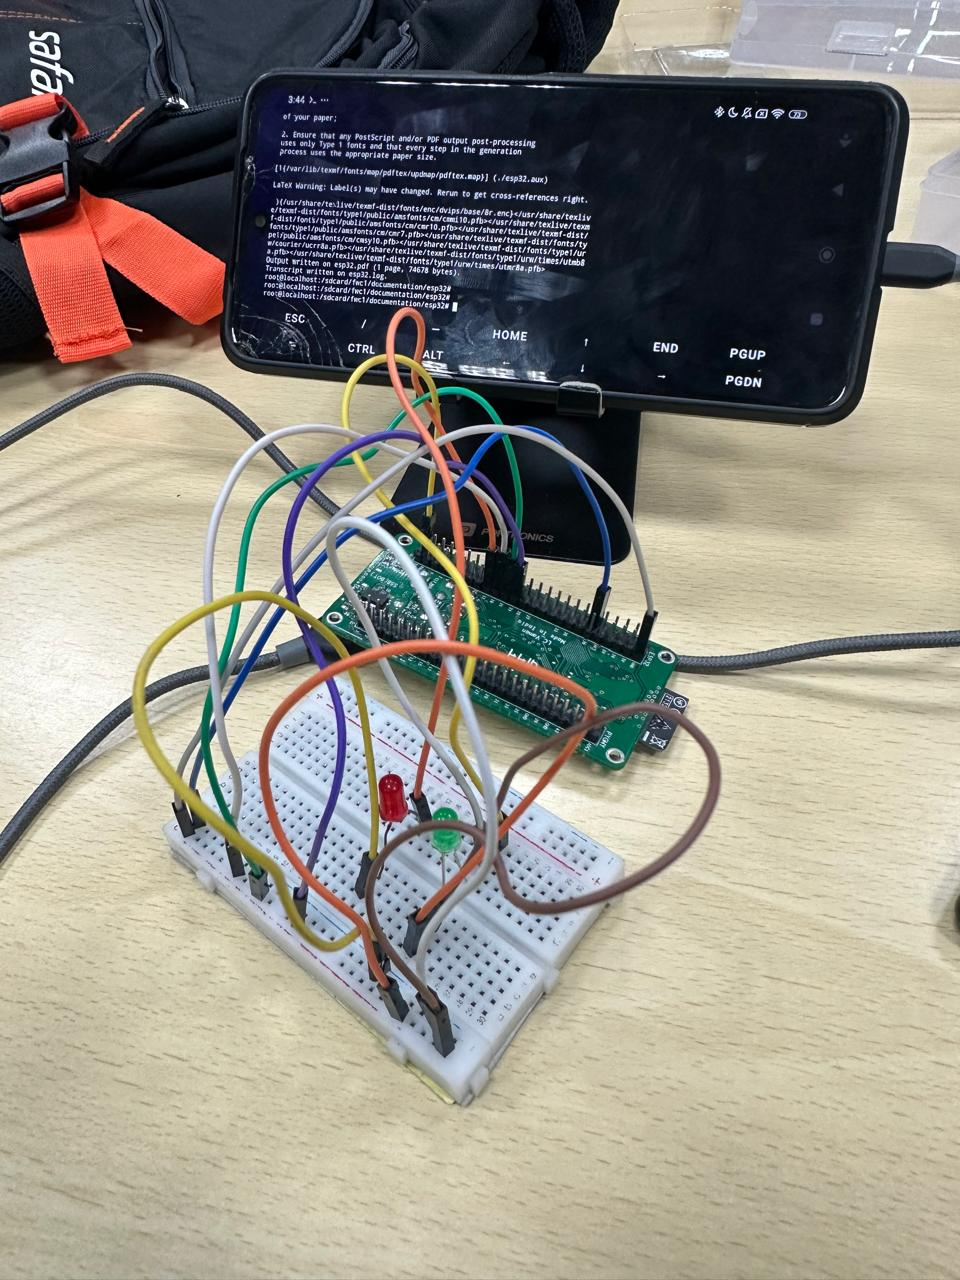
\includegraphics[width=0.25\textwidth]{espp.jpg}
	\caption{\label{fig:Gates}}    
\end{figure}
\newpage
\section{CONCLUSION}
Encoders play a critical role in a wide range of applications, offering precise and reliable data about position, speed, and direction. The ESP-32 on the vaman board is a versatile microcontroller with Wi-Fi, Bluetooth and extensive GPIO, ideal for IoT and embedded systems. Its integration with the vaman boards features makes it suitable for prototyping and deploying smart, connected projects. 

\end{document}
